\documentclass[10pt,twocolumn,letterpaper]{article}

\usepackage{cvpr}
\usepackage{times}
\usepackage{epsfig}
\usepackage{graphicx}
\usepackage{amssymb}
\usepackage{enumerate}
\usepackage{textcomp}
\usepackage{graphicx}
\usepackage{mathtools}
\graphicspath{ {images/} }

% Include other packages here, before hyperref.

% If you comment hyperref and then uncomment it, you should delete
% egpaper.aux before re-running latex.  (Or just hit 'q' on the first latex
% run, let it finish, and you should be clear).
\usepackage[breaklinks=true,bookmarks=false]{hyperref}

\cvprfinalcopy % *** Uncomment this line for the final submission

\def\cvprPaperID{****} % *** Enter the CVPR Paper ID here
\def\httilde{\mbox{\tt\raisebox{-.5ex}{\symbol{126}}}}

% Pages are numbered in submission mode, and unnumbered in camera-ready
%\ifcvprfinal\pagestyle{empty}\fi
\setcounter{page}{1}
\begin{document}

%%%%%%%%% TITLE
\title{EECS 442 Computer Vision: Final Project Report}

\author{Nathan Immerman\\
College of Engineering, University of Michigan\\
Ann Arbor, Michigan\\
{\tt\small immerman@umich.edu}
% For a paper whose authors are all at the same institution,
% omit the following lines up until the closing ``}''.
% Additional authors and addresses can be added with ``\and'',
% just like the second author.
% To save space, use either the email address or home page, not both
\and
Alexander Chocron\\
College of Engineering, University of Michigan\\
Ann Arbor, Michigan\\
{\tt\small achocron@umich.edu}
}

\maketitle
%\thispagestyle{empty}

%%%%%%%%% BODY TEXT
\section{Introduction}

With the advent of software tools such as Photoshop and Gimp, it is becoming increasingly simple to doctor and create fake images. One method of doctoring images is to create a composite image out of existing source images. Since composite images are difficult to detect for the common person, we hope to create a tool that enables users to determine composite images.

It is often difficult to make the light direction throughout the entirety of composite images consistent. This fact can be leveraged to detect whether even well-stitched images are fake. By analyzing the light direction of different surfaces within the image, one can detect whether or not the two surfaces came from the same original image. An algorithm for detecting such inconsistencies has been outlined in Johnson and Farid's paper, \emph{Exposing digital forgeries by detecting inconsistencies in lighting}. We shall attempt our own implementation of this algorithm and measure our implementation based on accuracy.
%------------------------------------------------------------------------
\section{Approach}

The equation that we are making use of to estimate the light directions is \[I(x,y) = R\times (\vec{N}(x,y)\cdot \vec{L}) + A\]
where $I(x,y)$ is the intensity at the point $(x,y)$, $R$ is the reflectance term (a constant), and $N(x,y)$ is the unit vector normal to the boundary at the point $(x,y)$. This equation assumes an infinite light source.

A limitation of this equation is that it requires that the reflectance of the surface is known and that it is constant. By assuming that the reflectance equals 1, a vector for the light direction can be obtained with an unknown scale factor. However, this still requires that the object has constant reflectance. As the paper suggests, we are able to relax this constraint by partitioning the boundary into $n$ patches, and assume that each of these patches has constant reflectance. The underlying assumption here is that more smaller, local patches of an object are likely to be most uniform, and therefore are likely to have a more constant reflectance than the entire object. In our implementation, we use $n$ = 8, which the authors of the paper recommend.

\subsection{Finding the Normal Vectors}
The algorithm assumes that the boundaries are given, but the equation we are using requires that the vectors normal to the object boundaries are calculated. The reason we do not consider an arbitrary point on an object is that we cannot easily estimate the normal vectors at these points. We already know that the z-component of the vector is equal to 0 on the object boundary, and the x and y components point in the same direction in both the scene and image coordinates at these points, making them very easy to estimate with no object-level knowledge or 3D information. We estimate a normal vector for each point given in every partition. But the boundary is given as a set of points, and it is clearly impossible to estimate the normal vectors of discrete, non-continuous function. To solve this, we begin by fitting a quadratic curve $y = p(x)$. The curve is fit to three user-selected points that lie near the boundary partition. We then observe each point $(a,b)$ in the partition, and find a unit-vector perpendicular to the quadratic curve at the point $(a,p(a))$. 

At each partition, the user must indicate a fourth point that lies on the object to indicate which direction the normal vectors should point. If the normal vector that we calculate points away from this point, we simply scale it by a factor of -1.

\subsection{Estimating intensities at the occluding boundary}
We need to estimate the intensities of the pixels at the occluding boundary because the pixels are not in the image. For a single point along the boundary, this is accomplished by sampling $n$ pixels along the direction opposite of the normal vector and fitting an exponential curve to these values, namely \[I(x) = ax^{b}\] where x is the position along the negative normal direction and $I(0)$ is the intensity at the occluding boundary. We used $n = 15$.

We use least-squares estimation on $\log(I(x))$ to determine the parameters $a$ and $b$. The intensity at the occluding boundary is then calculated by evaluating $I(0)$.

\subsection{Least Squares Solution}
We cannot take a direct approach to solving for the light directions; we have an unknown ambient term and several points in each partition segment. To overcome this, the paper reformulates the problem in such a way that it is possible to apply least squares estimation to solve for the unknowns. After this is complete, we estimate the overall light direction on the object by averaging the light direction of each segment in the partition.

The paper reformulates the problem by first organizing the data:

$(x^{(i)}_j,y^{(i)}_j)$ is the $j$th point of the $i$th partition for a particular boundary. There are $n$ partitions, each of which contains $p$ points.

$D_k = 
\begin{pmatrix}
N_x(x^{(1)}_1,y^{(1)}_1) & N_y(x^{(1)}_1,y^{(1)}_1) \\
	\vdots & \vdots\\
	N_x(x^{(1)}_p,y^{(1)}_p) & N_y(x^{(1)}_p,y^{(1)}_p) \\
	\end{pmatrix}$

	
$M = 
	\begin{pmatrix}
	D_1 & 0 &\cdots & 0 & 1\\
	0 & D_2 &\cdots & 0 & 1\\
 	\vdots & \vdots & \ddots & \vdots& \vdots\\
	0 & 0 & \cdots & D_n & 1\\
	\end{pmatrix}$
	
	
$C = 
	\begin{pmatrix}
	-1 & 0 & 1 & 0 & \cdots & 0 & 0 & 0 & 0 & 0\\
	0 & -1 & 0 & 1 & \cdots & 0 & 0 & 0 & 0 & 0\\
	\vdots & & & & \ddots & & & & & \vdots\\
	0 & 0 & 0 & 0 & \cdots & -1 & 0 & 1 & 0 & 0\\
	0 & 0 & 0 & 0 & \cdots & 0 & -1 & 0 & 1 & 0\\
	\end{pmatrix}$
	
$\vec{b} =
	\begin{pmatrix}
	I(x^{(1)}_1,y^{(1)}_1)\\
	\vdots\\
	I(x^{(1)}_p,y^{(1)}_p)\\
	\vdots\\
	I(x^{(n)}_1,y^{(n)}_1)\\
	\vdots\\
	I(x^{(n)}_p,y^{(n)}_p)\\
	\end{pmatrix}$


$\vec{v} = 
	\begin{pmatrix}
	L^{(1)}_x\\
	L^{(1)}_y\\
	\vdots\\
	L^{(n)}_x\\
	L^{(n)}_y\\
	A\\
	\end{pmatrix}$
	
$\vec{v}$ is the quantity we are trying to find. To do so, we use this closed form of the least squares optimization:

\[\vec{v} = (M^TM + \lambda C^TC)^+M^T\vec{b}\] where $A^+$ would denote the pseudo-inverse of $A$. This is the closed form equation for finding the least-squares estimate of the light directions.



%------------------------------------------------------------------------
\section{Implementation}

No third-party software or systems were used. All components of our project, including the back end and front end GUI (graphic user interface), were implemented from scratch (other than the built-in functions that MATLAB provides). We chose to implement our tool in MATLAB due to our familiarity with the software and its built-in linear algebra and image manipulation functionality.

\subsection{Back End}

\subsection{Front End GUI}
Since many aspects of our tool requires user input, we decided to make a MATLAB GUI to provided a pleasant experience for the user. The following are the steps that the user would take when using our tool. 

First, start the tool with the desired image as a command line argument. 

Second, add the occluding boundaries that the user wishes to determine the light direction of. To do this first we recommend zooming in on the occluding boundary by using the magnifying glass from the tool bar. Then click the button \emph{Add Boundary} and draw as close as possible to the occluding boundary while remaining on the actual object. The user should use the button \emph{Add Boundary} for each boundary that they wish to add. 

Third, once the user is done adding boundaries, the user should click the button \emph{Finish Boundaries}. In this phase of the tool, the user will be entering points that are used to estimate a quadric curve to fit to the boundaries that they user added. The GUI will zoom in on small patches of a boundary, the user should then enter three points that approximate the small patch. Then the user should enter an additional point that is on the object while remaining close to the patch. Once these four points are entered the GUI will zoom in on the next patch and the user should repeat the process until the user has entered four points for each patch on a boundary. 

Then the GUI will zoom out to reveal the entire boundary and the user should enter one point on the object where the user would like the estimated light direction to be plotted. This process will repeat for each boundary that the user added.

Once the user has completed entering all of these points, the GUI will plot the estimate light directions for each boundary at the locations that the user specified.

The user also has the ability to view the entered boundaries and the estimated normal vectors by toggling the buttons \emph{Toggle Boundaries} and \emph{Toggle Normal Vectors} respectively. 
% \begin{figure}[]
% \centering
%  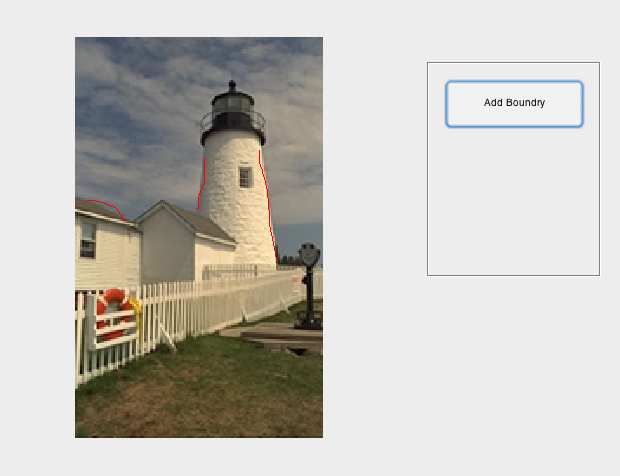
\includegraphics[scale=0.35]{gui_pic.png}
% \caption{Current State of our GUI, user selected boundaries in red}
% \label{GUI1}
% \end{figure}
%------------------------------------------------------------------------
\section{Experiments}
We performed a number of experiments to test the performance of our tool. These experiments included both testing the light direction of calculated in images for which a ground truth has been obtained, and testing the tool on known composits, with an emphasis on the former.
\subsection{Experiments with a known ground truth}
\begin{figure}[h]
\center
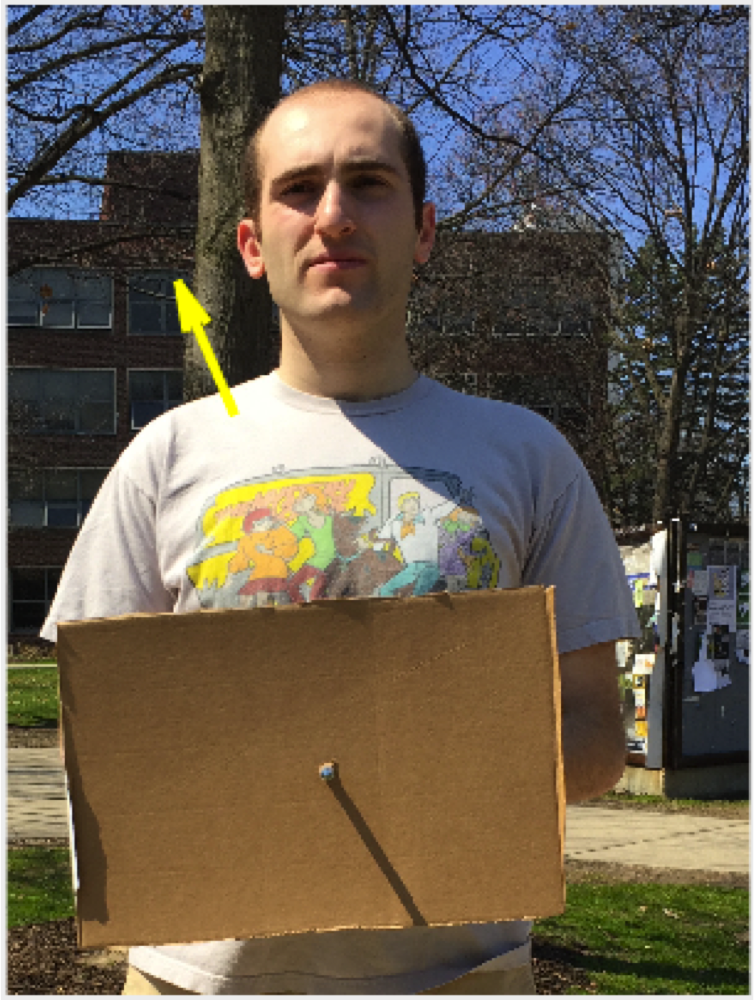
\includegraphics[scale = 0.3]{nathan.png}
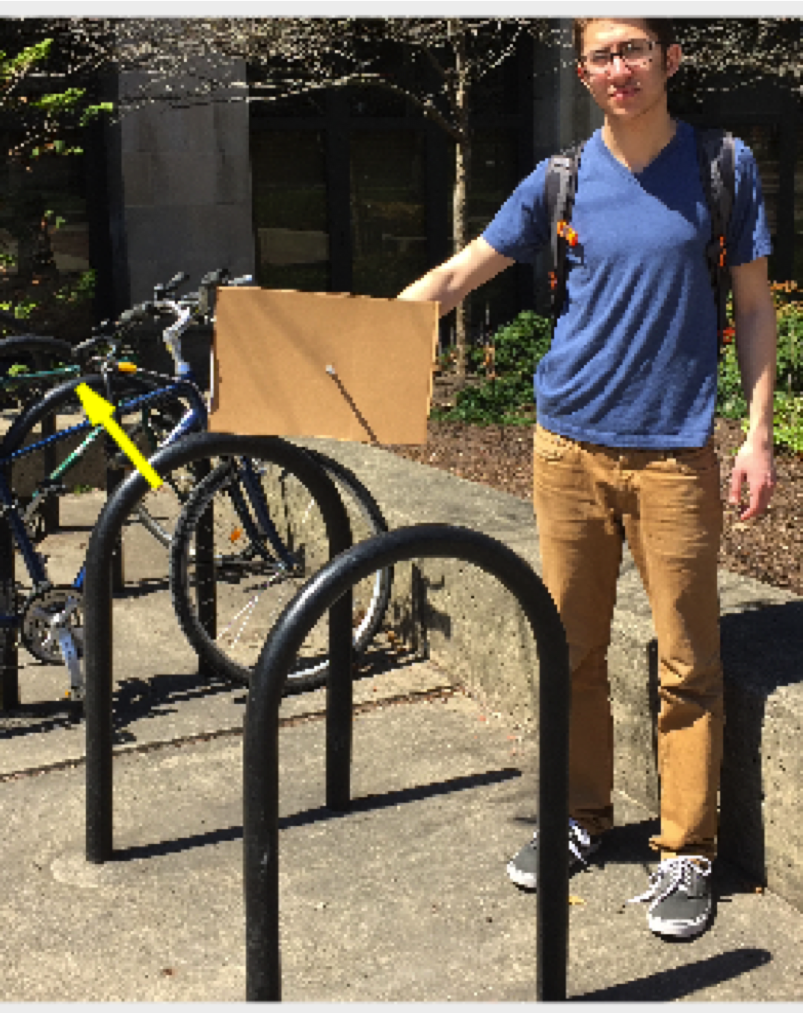
\includegraphics[scale = 0.3]{zander.png}
(a), (b)\\
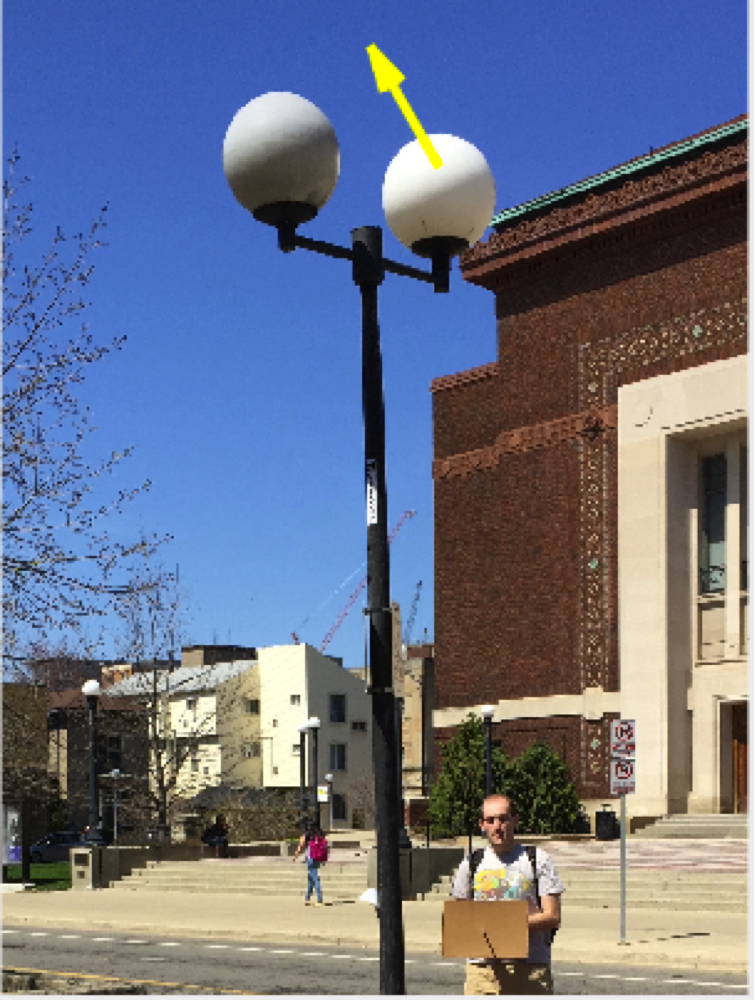
\includegraphics[scale = 0.3]{lamppost.png}
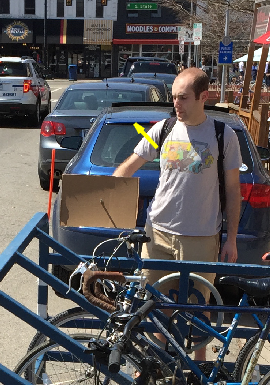
\includegraphics[scale = 0.374]{bike_rack_1.png}
(c),(d)\\
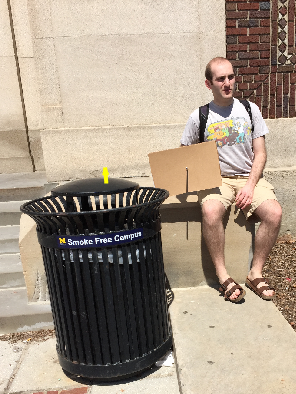
\includegraphics[scale = 0.35]{garbage_can.png}
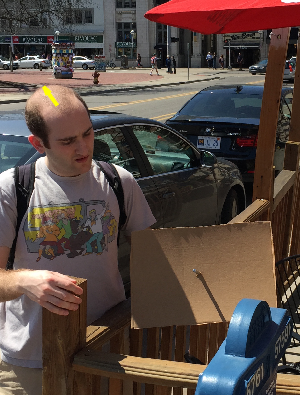
\includegraphics[scale = 0.35]{nathan_2.png}
(e),(f)
\end{figure}



IUFSLKDJNFLIUEJKSND are examples of images that we tested our tool on. The ground truth for the light direction was estimated by holding a board with a protruding rod parallel to the image plane and measuring the direction of the shadow cast by the sun. This was then compared to the output of our tool. A brief summary of our results:
\\\\
\begin{tabular}{c | c | c | c }

Image & Est. Direction & Ground Truth & Diff.\\
\hline
(a) & 121\textdegree & 113\textdegree & 8\textdegree\\
(b) & 122\textdegree & 128\textdegree & 6\textdegree\\
(c) & 115\textdegree & 120\textdegree & 5\textdegree\\
(d) & 133\textdegree & 120\textdegree & 13\textdegree\\
(e) & 95\textdegree & 89\textdegree & 6\textdegree\\
(f) & 126\textdegree & 119\textdegree & 7\textdegree\\
\end{tabular}
\\\\
Angles are measured South of West.
%------------------------------------------------------------------------
\section{Conclusion}

%--------------------------------	----------------------------------------
\section{References}

[1] M. K. Johnson and H. Farid. Exposing digital forgeries by detecting inconsistencies in lighting. \emph{In Proceedings of the 7th workshop on Multimedia and security}, pages 1-10, 2005.


\end{document}































